\documentclass[10pt,twocolumn,letterpaper]{article}

\usepackage{cvpr}
\usepackage{times}
\usepackage{epsfig}
\usepackage{graphicx}
\usepackage{amsmath}
\usepackage{amssymb}
\usepackage{subcaption}

% Include other packages here, before hyperref.

% If you comment hyperref and then uncomment it, you should delete
% egpaper.aux before re-running latex.  (Or just hit 'q' on the first latex
% run, let it finish, and you should be clear).
\usepackage[breaklinks=true,bookmarks=false]{hyperref}

\cvprfinalcopy % *** Uncomment this line for the final submission

\def\cvprPaperID{****} % *** Enter the CVPR Paper ID here
\def\httilde{\mbox{\tt\raisebox{-.5ex}{\symbol{126}}}}

% Pages are numbered in submission mode, and unnumbered in camera-ready
%\ifcvprfinal\pagestyle{empty}\fi
\setcounter{page}{1}
\begin{document}

%%%%%%%%% TITLE
\title{Supervised Learning of Semantic Word Embeddings from Semantic Entailment Data}

\author{Ao Liu\\
University of Massachusetts Amherst\\
140 Governors Dr., Amherst, MA 01003 \\
{\tt\small aoliu@umass.edu}
% For a paper whose authors are all at the same institution,
% omit the following lines up until the closing ``}''.
% Additional authors and addresses can be added with ``\and'',
% just like the second author.
% To save space, use either the email address or home page, not both
}

\maketitle
\begin{abstract}
Many natural language processing (NLP) tasks rely word embeddings. Traditionally, word embeddings are trained unsupervisedly on large corpus. This approach has in general worked well on many NLP related tasks. However, implementations of this unsupervised approach usually focus on the syntactic representations of words, thus lack of semantic interpretations. One of the problem is syntactic representations can hardly deal with negation and degree modifiers. Research shows that multiplicative embeddings perform better on semantic tasks, such as entailment. As an important task of semantics, entailment teaches the computer how to understand the meaning of a sentence and the implicit idea behind it. In this paper, I will show a supervised way to train multiplicative semantic word embeddings with the help of entailment dataset. Computer vision uses ImageNet to obtain features and then transfer them to other tasks. My work tends to indicate the capability of word embeddings trained on natural language inference to be transferred to other NLP tasks.
\end{abstract}

\section{Introduction}
Distributed representations of words (or word Embeddings)\cite{bengio2003neural, collobert2011natural, mikolov2013distributed, pennington2014glove} are generally used for many NLP tasks in recent years. Although these unsupervisedly trained word embeddings are capable of finding the general topic in a sentence based on the syntactic relationships of words, they still lack of semantic interpretations. Due to this problem, it is hard to find meaningful representation of a full sentence. A most recent paper shows that capturing the relationships among multiple words and phrases in a single vector to form the sentence representation can improve the performance on semantic entailment tasks \cite{conneau2017supervised}. However, the provided method using syntax-based word embeddings may still have ignored the impact of semantic meanings of words.

There are two major families of unsupervisedly learning wrod embeddings: 1) global matrix factorization methods, such as latent semantic analysis (LSA) \cite{deerwester1990indexing} 2) co-occurrence methods, such as skip-gram model of Mikolov  \cite{mikolov2013distributed} and global log-bilinear regression model of Pennington \etal \cite{pennington2014glove}. Pennington \etal seem better statistically solving global information, but the problem of semantics interpretation remain unsolved. Some significant examples are around 1) negation words, such as "not" and 2) degree modifiers, such as "more" and "less". Those examples are problematic because such negation words or degree modifiers can be added to any syntactically completed sentences, but the semantic meaning of the sentence may be altered for a certain degree. Training such words in an unsupervised manner is unwise and usually result in meaningless representations.

In my project, I try to study the task of learning semantic word embeddings that is trained on a large corpus in order to relieve some difficulties of finding more general semantic sentence representations. To obtain such semantic word embeddings, two major problem need to be solved, namely: what would be a suitable neural network architecture; and how and on what task should such a network be trained. Most approaches of existing work on learning word embeddings in an unsupervised maner like word2vec \cite{mikolov2013distributed} and GloVe \cite{pennington2014glove}. I want to see if supervised learning can help solving the problem. The idea is inspired by previous result in NLP, where Alexis Conneau \etal train universal sentence representation \cite{conneau2017supervised}, and in computer vision, where researchers pretrain models on the ImageNet \cite{deng2009imagenet} and transfer the learned features to other tasks. Conneau \etal show that training sentence encoders on a natural language inference (NLI) task achieve the best transferability \cite{conneau2017supervised}. The reason is that NLI is a high-level understanding task involving reasoning about the semantic relationships within sentences. Hence, I hypothesize that such task can also help training semantic word embeddings.

Unlike in computer vision, where convolutional neural networks (CNNs) dominate the field, many architectures are used in NLP tasks. Hence, I investigate different methods of training word embeddings with supervision, and compare their transferability to other task. My experiments show that the word embeddings recursively trained on the Stanford Natural Language Inference (SNLI) dataset \cite{bowman2015large} using the multiplicative trick yields better accuracies on  SNIL dataset and the Microsoft Research Paraphrase Corpus than sentence-encoder-based method introduced by Conneau \emph{et al} \cite{conneau2017supervised}.

\section{Related Work}
Transfer learning using supervised features trained on ImageNet \cite{deng2009imagenet} has been successful on various computer vision tasks \cite{sharif2014cnn}, such as face recognition \cite{taigman2014deepface} and visual question answering \cite{antol2015vqa}.

In contrast, most approaches of training word embeddings are unsupervised. This is mainly because people in NLP has not yet found the best supervised task for embedding the semantics of a word. With this reason, people compromise to unsupervised word embedding trained on large corpus, such as word2vec \cite{mikolov2013distributed} and Gloval Vectors (GloVe) \cite{pennington2014glove}, which both statistically capture the syntactic co-occurrence information among words.

One aproach of training word embeddings in an unsupervised manner is to learn word representations using local context windows. Bengio \etal \cite{bengio2003neural} introduced a model that learns word embeddings as a part of a neural network architecture for language modelling.

The skip-gram model of Mikolov \etal \cite{mikolov2013distributed} propose a simple single-layer architecture based on the inner product between two word vectors. In their model, the objective is to predict a word's context given the word itself. The skip-gram model show its capability of learning linguistic patterns as linear relationships between word vectors with the evaluation on a word analogy task. Pennington \etal better solve the problem by including global co-occurrence statistics.

However, unsupervised learning models makes it harder for the word embeddings to specialize on semantic tasks. Conneau \etal \cite{conneau2017supervised} show that co-adaptation of sentence encoders and classifiers, when trained end-to-end on SNLI dataset, doesn't impact the generalization power of sentence features generated by an encoder.

To my knowledge, this work is the first attempt to use the SNLI dataset to train semantic word embeddings. As I show in my experiments, I can outperform unsupervised word embeddings and supervised sentence encoders on selected tasks.

\section{Approach}
This work combines two research directions. First, I explain how the NLI task can be used to train semantic word embeddings using the SNLI task. Then I describe the architectures that I investigate for the embedding model and the entailment model. Specifically, for embedding model, I examine separated training of word embeddings and the end-to-end approach, and for entailment model I test different recurrent models such as gated recurrent units (GRU) \cite{chung2014empirical}, long short-term memory (LSTM) \cite{hochreiter1997long} and their bidirectional variants.

\subsection{The Natural Language Inference Task}
In SNLI, there are 570k human-written English sentence pairs labelled with one of the three categories: entailment, contradiction, and neutral. It captures NLI, or Recognizing Textual Entailment (RTE), and is one of the largest high-quality labelled dataset for semantics related NLP training purpose. I hypothesize that the semantic nature of NLI makes it a good candidate for learning semantic word embeddings in a supervised way. That is, I want to show that semantic word embeddings trained on NLI are able to capture the semantic meaning of words and can potentially improve the performance of entailment systems.

\subsection{Word Embedding Models}
There are two ways to train the word embeddings on SNLI: 1) adapt word co-occurrence statistics and 2) train embeddings of words in a sentence pair simultaneously.

\begin{figure}[t]
\begin{center}
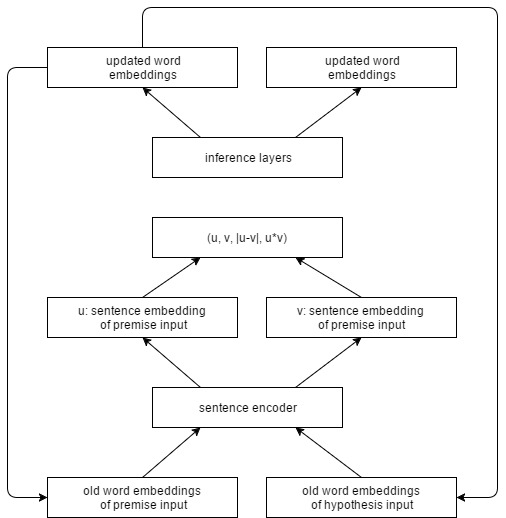
\includegraphics[scale=0.4]{model_architecture}
\end{center}
\caption{A generic architecture of learning word embeddings on SNLI in a supervised manner}
\label{fig:model_arc}
\end{figure}

Since training word embeddings within sentence pairs simultaneously implicitly shows the co-occurrences of words, I adopt the second setting. As illustrated in Figure \ref{fig:model_arc}, a typical architecture of this kind trains word embeddings of sentence pairs simultaneously. The word embeddings of premise and hypothesis inputs are passed through a shared sentence encoder to obtain the sentence embeddings premise $u$ and hypothesis $v$. Once the sentence embeddings are generated, 3 matching methods are applied to extract relations between $u$ and $v$: 1) concatenation of $u$ and $v$, 2) element-wise absolute difference $|u - v|$ and 3) element-wise product $u*v$. The resulting vector will contain informations from both $u$ and $v$ and then be passed into inference layer(s) along with a softmax output layer. This will simultaneously update all the embeddings of words in the sentence pair and the updated word embeddings will then be applied to the following training iterations.

\subsubsection{Pre-train Word Embeddings}
In this setting, I hypothesize that sentence representation can be formed by the Cartesian point-wise multiplication of word embeddings. That is, a sentence $s = [w_1, ..., w_N]$ of length $n$ has the vector representation $v_s$ of the form $v_s = v_{w_1} \times ... \times v_{w_N}$, where $v_{w_n}$ is the word embedding of $n$-th word in the sentence $s$. Thus, for a sentence pair, the division will result in $1$ for entailment label and $-1$ for contradiction label, \ie $u / v = 1$ for entailment and $u / v = -1$ for contradiction.

Then the model is only trained on sentence pairs with entailment and contradiction labels to obtain the pre-trained word embeddings.

\subsubsection{End-to-End Approach}
In this setting, I adopt the same hypothesis of embedding multiplication from the pre-trained model. In addition, the model is also trained on the traditional entailment architecture simultaneously so that the model jointly learns the word embeddings and the entailment model.

\subsection{Entailment Model}
Various neural networks for NLI exist. However, current systems are usually based on pre-trained word embeddings using unsupervised techniques. The architecture that better fits the semantic word embeddings is not yet clear. Thus, I compare different architectures: GRU- and LSTM- based models, and their bidirectional variants.

\section{Datasets}
I only choose two datasets. One is the SNLI dataset \cite{bowman2015large}, where I train the word embeddings. The other one is the Microsoft Research (MSR) Paraphrase Corpus \cite{dolan2004unsupervised}, where I evaluate the transferability of the word embeddings trained on the SNLI dataset. Data samples are shown in Table \ref{tab:data_sample}.

\subsection{The SNLI Dataset}
The SNLI dataset is a collection of 570k human-written English sentence pairs manually labeled for balanced classification with the labels entailment, contradiction, and neutral, supporting the task of natural language inference (NLI), also known as recognizing textual entailment (RTE). 

\subsection{The MSR Paraphrase Corpus}
The MSR Paraphrase Corpus contains 5.8k sentence pairs obtained from a corpus of temporally and
topically clustered news articles collected from thousands of web-based news sources using unsupervised techniques. For each sentence pair, the relation would be either true or false paraphrase.

\begin{table*}
\begin{center}
\begin{tabular}{|l|c|l|l|c|}\hline
Dataset		& size	& premise	& hypothesis	& label \\\hline
SNLI		& 570k	& A man inspects the uniform of a & The man is sleeping. & neutral\\
&					& figure in some East Asian country.	&&\\
			& 		& An older and younger man smiling.	& Two men are smiling and laughing & neutral\\
			&		&		& at the cats playing on the floor. &\\
			& 		& Some men are playing a sport.	& Some men are playing a sport. & entailment\\\hline
MSR			& 5.8k	& Ricky Clemons' brief, troubled & Missouri kicked Ricky Clemons off its & True\\
Pharaphrase &		& Missouri basketball career is over. & team, ending his troubled career there. &\\
Corpus	&			& Russ Britt is the Los Angeles Bureau & Emily Church is London bureau chief & False\\
&					& Chief for CBS.MarketWatch.com. & of CBS.MarketWatch.com. &\\\hline
\end{tabular}
\end{center}
\caption{\textbf{Data samples.} The SNLI dataset has labels of entailment, contradiction and neutral. The MSR Paraphrase Corpus only has labels of true and false paraphrase.}
\label{tab:data_sample}
\end{table*}

\begin{figure*}
\centering
\begin{subfigure}{.5\textwidth}
  \centering
  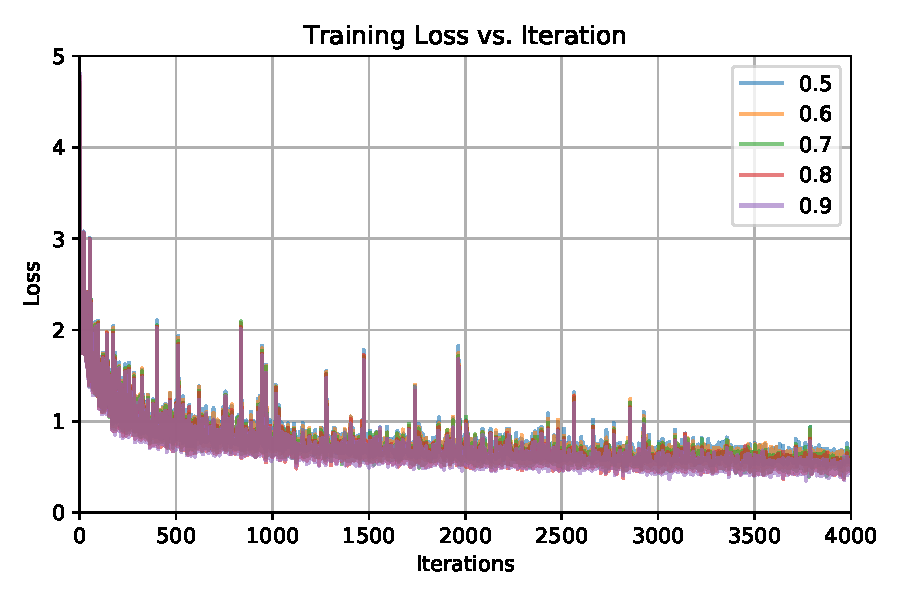
\includegraphics[scale=0.45]{train_loss}
  \label{fig:train_loss}
\end{subfigure}%
\begin{subfigure}{.5\textwidth}
  \centering
  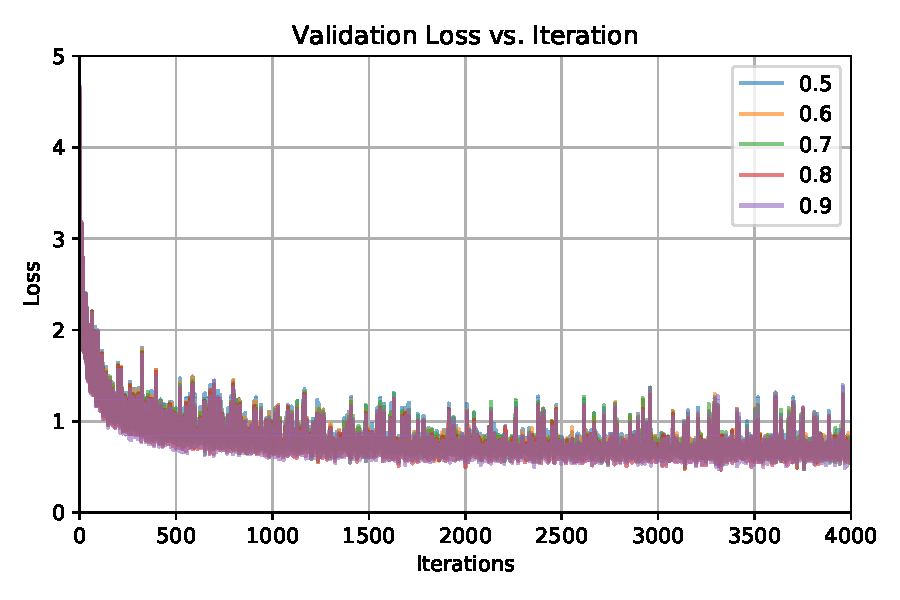
\includegraphics[scale=0.45]{dev_loss}
  \label{fig:dev_loss}
\end{subfigure}
\caption{Training and validation loss on SNLI dataset.}
\label{fig:loss}
\end{figure*}

\begin{figure*}
\centering
\begin{subfigure}{.5\textwidth}
  \centering
  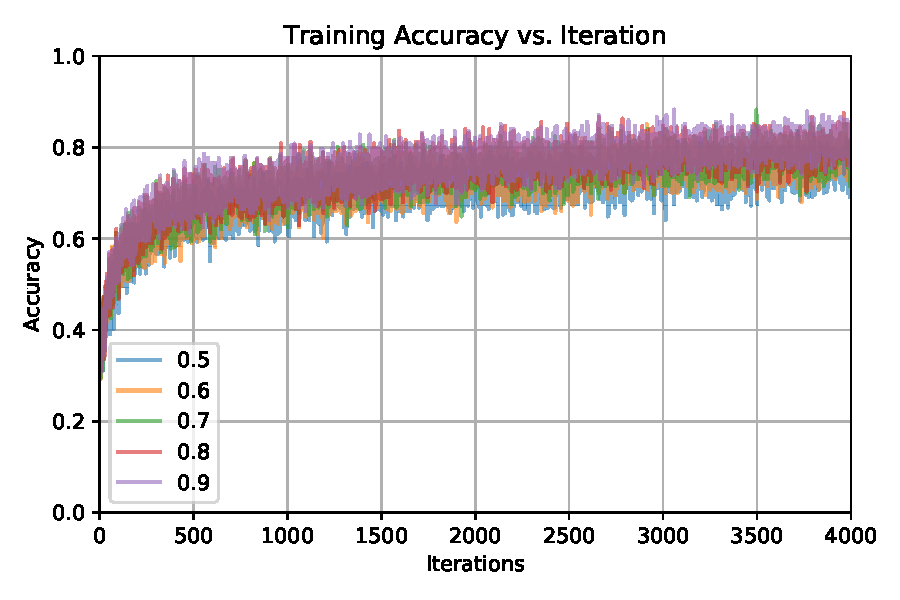
\includegraphics[scale=0.45]{train_acc}
  \label{fig:train_acc}
\end{subfigure}%
\begin{subfigure}{.5\textwidth}
  \centering
  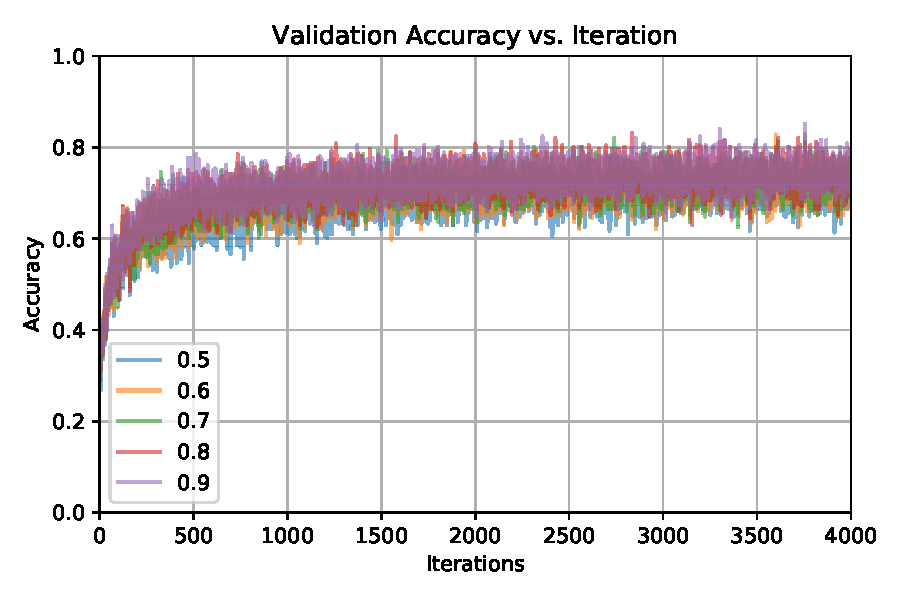
\includegraphics[scale=0.45]{dev_acc}
  \label{fig:dev_acc}
\end{subfigure}
\caption{Training and validation acc on SNLI dataset.}
\label{fig:acc}
\end{figure*}

\begin{table*}
\centering
\begin{center}
\begin{tabular}{|l|c|c|c|c|}\hline
Model		& dim	& SNLI dev	& SNLI test	& MSR test \\\hline
LSTM		& 2048	& 81.9	& 80.7	& 79.5 \\\hline
GRU			& 4096	& 82.4	& 81.8	& 81.7 \\\hline
BiGRU-last	& 4096	& 81.3	& 80.9	& 82.9 \\\hline
BiLSTM-Mean	& 4096	& 79.0	& 78.2	& 83.1 \\\hline
BiLSTM-Max	& 4096	& 85.0	& 84.5	& \textbf{85.2} \\\hline
BiLSTM(pre-trained embedding	& \textbf{512}	& 83.6	& 83.1	& 83.4 \\
with multiplication trick) (\textbf{my model})&&&&\\\hline
BiLSTM with multiplication trick (\textbf{my model})	& \textbf{512}	& \textbf{85.2}	& \textbf{84.7}	& \textbf{85.2} \\\hline
\end{tabular}
\end{center}
\caption{Accuracies of SNLI development and test datasets, and accuracies of the transfer task MSR Pharaphrase Corpus. The dimension column indicates the number of hidden units of the sentence encoder. The performances of the first five models are provided by Conneau \etal \cite{conneau2017supervised}.}
\label{tab:acc}
\end{table*}

\section{Experiments}
My goal is to obtain general-purpose word embeddings that capture semantic information that can be transferred to other tasks. To evaluate the quality of the word embeddings trained on the SNLI dataset with the multiplication trick, I use them as features on MSR Paraphrase Corpus. I present my procedure of evaluating the word embeddings in this section.

\subsection{Evaluation Method}
Traditional evaluation on the quality of word embeddings are in three categories: 1) word analogy task, 2) word similarity task and 3) downstream NLP tasks, such as named entity recognition (NER). The word analogy task is to find the missing word $b^*$ in the relation: $a$ is to $a^*$ as $b$ is to $b^*$, where $a$, $a^*$ are related by the same relation as $b$, $b^*$. A classic example is $king : man :: queen : woman$ \cite{mikolov2013distributed}. Recent research show that solving this problem is equivalent to computing a linear combination of word similarities between the query word $b^*$, with the given word $a$, $a^*$ and $b$ \cite{levy2014linguistic}. However, Faruqui \etal found there is a problem with similarity-based evaluation of word embeddings \cite{faruqui2016problems}. That is, using word similarity task for evaluation of word embeddings may lead to incorrect inferences. Furthermore, they suggest task specific evaluation. For the purpose of finding better semantic word embeddings, I evaluate  the performance of the word embeddings on the original SNLI dataset and the MSR Paraphrase dataset. The preferred evaluation metric for both of tasks is accuracy, since the two tasks are either 3-way classification or binary classification problem.

\subsection{Training Details}
Since SNLI dataset has pre-split training, development and test datasets, I train my model on the training set, which contains 550k sentence pairs. I tokenize and lowercase the dataset with NLTK's word tokenizer, and build a vocabulary of 30k most frequent words.

For my experiments, I train the model using Adam optimization algorithm \cite{kingma2014adam}. Since Adam using adaptive learning rate, I choose a reasonable starting learning rate, $3e-3$. I use the early-stop trick to test convergence, where there is no decrease in the loss of development set for the last 500 iterations. To compare with the performance of entailment system by Conneau \etal \cite{conneau2017supervised}, I choose the same dimension of word embeddings as 300, which they adopt the pre-trained GloVe word embeddings, and the same number of hidden units of the inference layer as 512. I choose the mini-batch size as 256 for training. I use 512 hidden states for bi-LSTMs sentence encoder to save time for the purpose of course project. The dropout rate is chosen based on the performance on the development dataset of SNLI through cross-validation.

\subsection{Results}

\subsubsection{Dropout Impact}
To choose the best inverse dropout rate, I cross-validate the values of $[0.5, 0.6, 0.7, 0.8, 0.9]$. Figure \ref{fig:loss} shows the training and validation losses during the training process, and Figure \ref{fig:acc} shows the corresponding accuracies. The graph shows that when the inverse dropout rate is $0.9$, I obtain the best trade-off between training loss and validation loss. And the model achieves the best accuracy of $85.2\%$ on the development dataset of SNLI.

\subsubsection{Transferability}
From Table \ref{tab:acc}, we can see that my model, which uses Bi-LSTM of only 512 hidden units with multiplication trick, achieves the best accuracies of $85.2\%$ and $84.7\%$ on the development and test datasets of SNLI correspondingly. It also performs equally with the Bi-LSTM-Max model of Conneau \etal when transfers to MSR Paraphrase Corpus and gets accuracy of $85.2\%$.

\section{Conclusions}
This paper studies the effects of training semantic word embeddings with supervised data by transferring to another semantic task. My results shows that my word embedding model trained on SNLI dataset can perform better than models trained with pre-trained unsupervised word embeddings. With word embeddings trained using the multiplication trick, a simple Bi-LSTM sentence encoder outperforms the complex Bi-LSTM-Max sentence encoding method of Conneau \etal.

I believe that my work only scratches the surface of possible models for learning semantic word embeddings. Larger datasets of semantics could improve the quality of semantic word embeddings.

Future work may fall into two categories. One way is to test the performance of the trained word embeddings on other semantic tasks, such as Semantic Textual Similarity. The other is to find better model of training such embeddings. Due to the time we have for the course project, I did not explore much more other possible architectures.

\bibliographystyle{unsrt}
\bibliography{report}
\end{document}
